% !TEX program = xelatex
\documentclass{misisarticle}
\usepackage{float}

\grnti{28.23.15, 28.23.37}
\asjc{1707, 1702}
\oecd{01.02.EP}

\title{Сравнение моделей монокулярной оценки глубины без дообучения по геометрическим критериям}

\misisauthor{Егоров Ф. Д.}{кафедра инженерной кибернетики НИТУ «МИСиС»}{Москва, Россия}{m2514205@edu.misis.ru}

\setabstract{Монокулярные модели оценки глубины, обученные на смеси разнородных наборов данных, позволяют получить карту глубины по одному снимку без дообучения на целевой сцене, что делает их привлекательными для задач трёхмерного компьютерного зрения при отсутствии стереопары или лидара. В работе сравнивается точность и производительность моделей оценки глубины MiDaS, Depth Anything V2, Metric3D v2 и UniDepth V2 на наборе NYU Depth v2 при трёх процедурах согласования, а также по геометрическим критериям, вычисляемым на облаке точек, полученном обратным проецированием карты глубины.}
\setkeywords{трёхмерное компьютерное зрение, монокулярная оценка глубины, облако точек, попиксельная оценка.}

\begin{document}

\maketitle

\section{Введение}

Большинство прикладных задач трёхмерного компьютерного зрения --- навигация мобильных роботов \cite{pub6} и автономного транспорта \cite{pub7}, захват объектов манипулятором, измерение габаритов груза, восстановление планировок помещения \cite{pub8}, дополненная реальность --- требуют знания расстояния от камеры до точек сцены. Чаще всего на практике карты глубины получают с использованием дополнительного оборудования, например стереопары или лидара \cite{pub9}. Такое оборудование повышает стоимость и сложность системы, требует калибровки и настройки, а также имеет ограничения по дальности, освещению и типу поверхности: стереоалгоритмы не работают на однородных, плоских поверхностях, оптические датчики дают ошибку на зеркальных или прозрачных объектах. Обычные RGB-камеры уже присутствует в большинстве систем и работают в широком диапазоне условий, поэтому оценка глубины сцены по одному снимку представляет непосредственный практический интерес.

Задача восстановления глубины по одному изображению поставлена некорректно: сцена и её копия, увеличенная в произвольное число раз и отодвинутая от камеры на соответствующее расстояние, дают одинаковое изображение. Наблюдаемое изображение определяет глубину лишь с точностью до неизвестного масштаба, а при неизвестных параметрах камеры --- с точностью до аффинного преобразования. Модели, обученные на одном наборе данных с известным сенсором, восстанавливают абсолютные расстояния, но опираются на статистику конкретного окружения (улица, склад, жилое помещение), и при смене обстановки или параметров камеры качество существенно ухудшается.

На практике это компенсируется обучением на смеси наборов данных, полученных из разных источников в разнообразном окружении, а модель вместо абсолютного значения обучается предсказывать величину, инвариантную к масштабу и сдвигу. Несогласованность источников устраняется видом функции потерь \cite{pub1}. Такие модели переносятся на новые сцены без дообучения, что обозначается термином «zero-shot». В дальнейшем их точность может быть улучшена путём повышения объёма и качества обучающих данных \cite{pub2} и передачи параметров камеры в модель для получения абсолютного масштаба\cite{pub3}, \cite{pub4}.

Нет однозначного подхода к оценке таких моделей: Большинство метрик вычисляются попиксельно после согласования предсказания с эталоном, и результат зависит от выбранной процедуры согласования: подбор масштаба и сдвига по эталону скрывает часть ошибки, а отсутствие согласования делает несравнимыми модели, предсказывающие относительную и абсолютную глубину. Кроме того, попиксельные метрики нечувствительны к искажению формы: карта глубины с малой относительной ошибкой может при обратном проецировании давать облако точек, в котором плоская стена выгнута, или углы между плоскостями грубо искажены. В прикладных задачах обычно рассматриваются облака точек и возникает необходимость распознавания плоскостей, поэтому при оценке модели разумно будет рассмотреть метрики, оценивающие величину крупных геометрических искажений.

Целью работы является сравнение современных монокулярных моделей оценки глубины по двум группам критериев: попиксельным метрикам с использованием трёх процедур согласования и геометрическим характеристикам облака точек, полученного обратным проецированием предсказанной карты глубины. Дообучение моделей не производится: модели запускаются с теми весами, которые были представлены авторами в их работах.

\section{Обзор методов}

Модель MiDaS \cite{pub1} ввела схему обучения на объединении наборов данных, полученных из разных источников: стереопары, лидарных данных, структурированной подсветки и метода structure from motion. Разметка этих источников выражена в разных единицах и имеет разное начало отсчёта, поэтому прямое сравнение предсказания с эталоном невозможно. Для разрешения этого используется функция потерь, инвариантная к масштабу и сдвигу: перед вычислением ошибки предсказание приводится к эталону аффинным преобразованием в пространстве обратной глубины. Модель предсказывает относительную глубину объектов и тем самым не вычисляет абсолютных расстояний.

Depth Anything V2 \cite{pub2} также предсказывает относительную глубину, но имеет иной состав обучающей выборки: размеченные реальные снимки заменены синтетическими, у которых разметка более точна и содержит тонкие детали, а покрытие реальных сцен обеспечивается большим массивом изображений с автоматической разметкой, полученной от крупной модели-учителя. Авторами опубликовано семейство моделей разного размера, а также варианты, дообученные для предсказания абсолютной глубины для внутренних и уличных сцен.

Metric3D v2 \cite{pub3} решает задачу восстановления абсолютного масштаба. Причина его неопреденности --- различие фокусных расстояний: один и тот же объект при использовании разных оптических систем занимает различное число пикселей, из-за чего одинаковые изображения соответствуют разным расстояниям. Авторы используют преобразование к канонической камере: изображение и разметка приводятся к общему фокусному расстоянию, модель работает в этом пространстве, а предсказание пересчитывается обратно по параметрам исходной камеры. Дополнительно модель предсказывает нормали к поверхности, согласованные с глубиной.

UniDepth \cite{pub4} использует близкую по смыслу идею, но параметры камеры не считаются известными: отдельный модуль предсказывает их по изображению, а выход представлен в псевдосферических координатах, что разделяет оценку направления луча и оценку расстояния вдоль него. Модель выдаёт непосредственно облако точек в метрических единицах.

Для оценки в помещениях повсеместно используется набор NYU Depth v2 \cite{pub5}, содержащий кадры RGB-D, снятые датчиком со структурированной подсветкой, с известными параметрами камеры. Все перечисленные работы приводят результаты тестирования на нём, однако процедуры согласования, области кадра и способы восстановления пропусков в эталоне у них различаются, что затрудняет прямое сопоставление опубликованных чисел. Настоящая работа не предлагает новых моделей и ограничивается сравнением существующих в едином протоколе.

\section{Постановка эксперимента}

\subsection{Набор данных}

Использована тестовая часть разбиения Eigen набора NYU Depth v2 \cite{pub5}: 654 кадра размеченного подмножества с разрешением 640$\times$480 пикс. Попиксельные метрики вычисляются только в центральной области изображения полученной срезанием 16 пикселей с каждого из краёв изображения, так как по краям модель не выдаёт значимых предсказаний. Эталоном для попиксельных метрик служит карта глубины с восстановленными пропусками (depths); для построения эталонных плоскостей используется исходная карта датчика (rawDepths), пиксели с пропусками исключаются. Учитываются пиксели с эталонной глубиной в интервале (0,001; 10) м, предсказания ограничиваются тем же интервалом. Пример кадра и соответствующей карты глубины приведён на рис. \ref{fig:nyu}.

\begin{figure}[H]
  \centering
  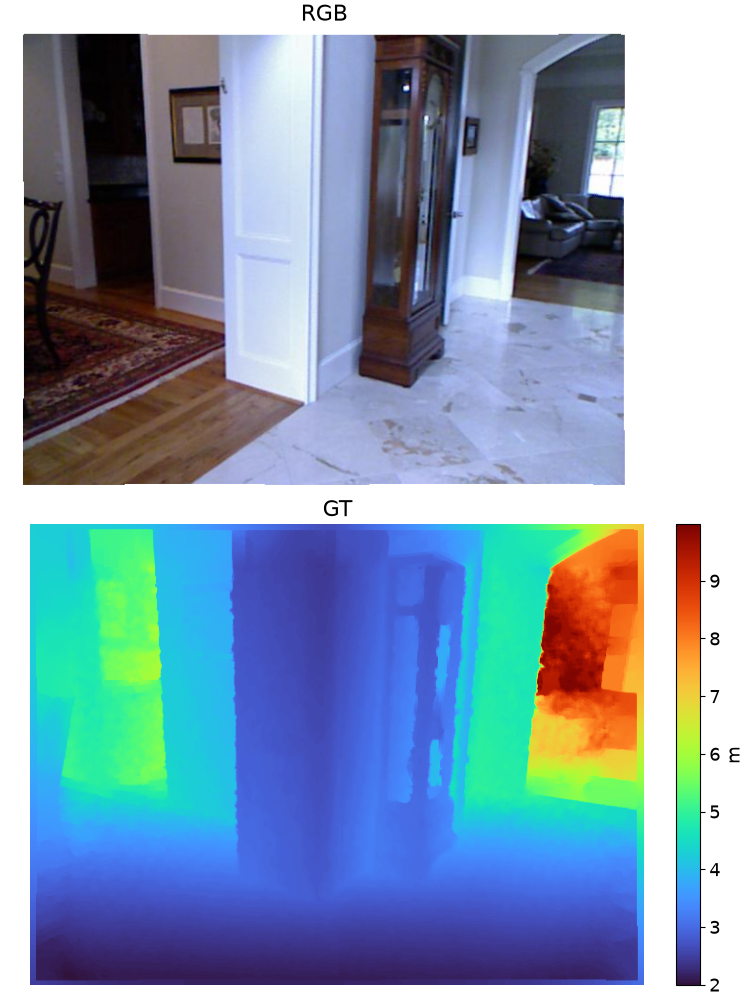
\includegraphics[width=0.73\columnwidth]{fig1.png}
  \caption{Кадр из тестовой выборки NYU Depth v2: RGB-изображение и эталонная карта глубины.}
  \label{fig:nyu}
\end{figure}

\subsection{Сравниваемые модели}

Производится сравнение следующих архитектур моделей: MiDaS v3 DPT-Hybrid, Depth Anything V2 Small, Metric3D v2 ViT-Small, UniDepth V2 Small. Metric3D v2 и UniDepth V2 также получают эталонные параметры камеры. Для инференса UniDepth V2 используется точность float16, остальных моделей --- float32.

\begin{table}[H]
  \caption{Сравниваемые модели}
  \label{tab:models}
  \centering
  \footnotesize
  \setlength{\tabcolsep}{3pt}
  \begin{tabular}{llcp{2.1cm}}
    \toprule
    \textbf{Модель} & \textbf{Вариант} & \textbf{\shortstack{Параметры,\\млн}} & \textbf{Тип предсказания} \\
    \midrule
    MiDaS & DPT Hybrid & 123,1 & относит. обратная глубина \\
    Depth Anything V2 & Small & 97,5 & относит. обратная глубина \\
    Metric3D v2 & ViT Small & 37,5 & глубина, м \\
    UniDepth V2 & Small & 114,4 & глубина, м \\
    \bottomrule
  \end{tabular}
\end{table}

\subsection{Аппаратное и программное обеспечение}

Эксперимент выполнен на компьютере с процессором AMD Ryzen 5 3600 (6 ядер, 12 потоков), 8 ГБ оперативной памяти и ускорителем NVIDIA A400 (4 ГБ видеопамяти). Для экспериментальных скриптов использовался язык программирования Python.

\subsection{Порядок эксперимента}

Для каждого кадра изображение uint8 загружается в память ускорителя; модель выполняет предобработку, инференс и приведение предсказания к разрешению 640$\times$480 пикс. Затем для каждой применимой процедуры согласования вычисляются попиксельные метрики, выполняется обратное проецирование и вычисляются геометрические характеристики.

Время вывода измеряется для каждого кадра при размере батча 1, от передачи изображения модели до получения карты глубины 640$\times$480 пикс., с синхронизацией CUDA до и после вызова; чтение с диска и копирование в память ускорителя не учитываются. Перед замером выполняется прогрев с помощью 10 запусков. Частота кадров FPS рассчитывается как $1000/t$, где $t$ --- среднее время инференса в мс. Потребление памяти ускорителя оценивается двумя величинами: пиковым объёмом, выделенным PyTorch за время загрузки модели и инференса, и объёмом, занятым процессом по данным вывода nvidia-smi во время инференса..

\section{Метрики и процедуры согласования}

Пусть $d$ --- предсказанная глубина, $d^*$ --- эталонная, $N$ --- число пикселей с известным эталоном. Использованы три общепринятые метрики: средняя относительная ошибка \eqref{eq:absrel}, среднеквадратичная ошибка \eqref{eq:rmse} и доля пикселей, у которых отношение предсказания к эталону не превышает порога 1,25 \eqref{eq:delta}.

\begin{equation}
  \mathrm{AbsRel} = \frac{1}{N}\sum \frac{|d - d^*|}{d^*}
  \label{eq:absrel}
\end{equation}
\begin{equation}
  \mathrm{RMSE} = \sqrt{\frac{1}{N}\sum (d - d^*)^2}
  \label{eq:rmse}
\end{equation}
\begin{equation}
  \delta_1 = \frac{\left|\left\{\max(d/d^*,\, d^*/d) < 1{,}25\right\}\right|}{N}
  \label{eq:delta}
\end{equation}

Все три метрики вычисляются после приведения предсказания к эталону. Рассмотрены три процедуры согласования: Первая --- согласование отсутствует; она применима только к моделям, предсказывающим абсолютную глубину, и оценивает восстановленный масштаб. Вторая --- умножнене на константу, подбираемую так, чтобы медианные расстояния на двух кадрах совпали \eqref{eq:median}; она устраняет ошибку масштаба, сохраняя ошибку формы. Третья --- масштабирование с параллельным переносом, параметры которого определяются методом наименьших квадратов в пространстве обратной глубины $x = 1/d$ \eqref{eq:lsq}; она принята при оценке моделей с относительным выходом и снимает как масштаб, так и сдвиг.

\begin{equation}
  s = \frac{\operatorname{median}(d^*)}{\operatorname{median}(d)}
  \label{eq:median}
\end{equation}
\begin{equation}
  (s, t) = \operatorname*{arg\,min}_{s,t} \sum (s x + t - x^*)^2
  \label{eq:lsq}
\end{equation}

Подбор параметров выполняется независимо для каждого кадра. Сравнение одной и той же модели при разных процедурах показывает, какая доля итоговой точности зависит от метода согласования, а не обобщающей способности модели. Для моделей с относительным выходом множитель \eqref{eq:median} вычисляется для обратной глубины; согласованная обратная глубина при процедурах \eqref{eq:median} и \eqref{eq:lsq} ограничивается снизу значением 0,1 м$^{-1}$.

\section{Геометрическая оценка}

Попиксельные метрики усредняют ошибку по кадру и не различают шумовое искажение всей поверхности и её изгиб или наклон, хотя для прикладных задач эти случаи неравноценны. Для их разделения карта глубины переводится в облако точек обратным проецированием \eqref{eq:backproj} с использованием известных параметров камеры, после чего оцениваются характеристики, инвариантные к общему масштабу и положению.

\begin{equation}
  \begin{aligned}
    X &= (u - c_x)\, d / f_x, \\
    Y &= (v - c_y)\, d / f_y, \\
    Z &= d
  \end{aligned}
  \label{eq:backproj}
\end{equation}

\subsection{Отклонение от плоскости}

Для каждого кадра в наборе данных также существует разметка с instance-сегментацией, включающая в себя такие заведомо плоские объекты, как пол, потолок, и стены. Таким образом, обратно спроецированные точки, покрываемые их масками, можно считать за отдельные плоскости и определить для них степень искажения. Для каждого плоского участка по точкам предсказанного облака методом RANSAC (256 гипотез, порог 3 см) строится плоскость, которая уточняется методом наименьших квадратов по точкам, лежащим в пределах порога; $\mathbf{n}$ --- единичная нормаль плоскости, $c$ --- её смещение. Отклонение от плоскости \eqref{eq:sigma} --- среднее расстояние до плоскости $K = 1000$ случайно выбранных точек участка, отнесённое к характерному размеру участка $L$, оцененному как среднее двух наибольших величин диапазонов координат $X$, $Y$, $Z$, покрываемых точками участка.

\begin{equation}
  \sigma = \frac{1}{K}\sum_{i=1}^{K} \frac{|\mathbf{n}^{\top}\mathbf{p}_i + c|}{L}
  \label{eq:sigma}
\end{equation}

Участок считается корректным, если содержит не менее $N = 3000$ пикселей и не менее 80\% его точек лежат в пределах порога; дальнейшие вычисления выполняются на этих пикселях. Всего было отобрано 1265 участков на 654 кадрах набора данных.

\subsection{Ошибка ориентации плоскости}

Для каждого плоского участка вычисляется угол между нормалью эталонной плоскости $\mathbf{n}^*$ и нормалью плоскости $\mathbf{n}$, построенной по предсказанному облаку на тех же пикселях \eqref{eq:angle}.

\begin{equation}
  \Delta\varphi = \arccos\left|\mathbf{n}^{\top}\mathbf{n}^*\right|
  \label{eq:angle}
\end{equation}

\section{Результаты}

В таблицах ниже приведены результаты измерения метрик для всех 3-х вариантов процедуры согласования, а также измеренное потребление памяти и времени моделями.

\begin{table}[H]
  \caption{Метрики без согласования}
  \label{tab:none}
  \centering
  \footnotesize
  \setlength{\tabcolsep}{3pt}
  \begin{tabular}{lccccc}
    \toprule
    \textbf{Модель} & \textbf{AbsRel} & \textbf{RMSE, м} & \textbf{$\delta_1$} & \textbf{$\sigma$, \%} & \textbf{$\Delta\varphi$, град.} \\
    \midrule
    MiDaS & --- & --- & --- & --- & --- \\
    Depth Anything V2 & --- & --- & --- & --- & --- \\
    Metric3D v2 & 0,091 & 0,363 & 0,928 & 0,549 & 5,3 \\
    UniDepth V2 & \textbf{0,082} & \textbf{0,329} & \textbf{0,943} & \textbf{0,404} & \textbf{3,5} \\
    \bottomrule
  \end{tabular}
\end{table}

\begin{table}[H]
  \caption{Метрики при согласовании по отношению медиан}
  \label{tab:median}
  \centering
  \footnotesize
  \setlength{\tabcolsep}{3pt}
  \begin{tabular}{lccccc}
    \toprule
    \textbf{Модель} & \textbf{AbsRel} & \textbf{RMSE, м} & \textbf{$\delta_1$} & \textbf{$\sigma$, \%} & \textbf{$\Delta\varphi$, град.} \\
    \midrule
    MiDaS & 0,347 & 1,643 & 0,492 & 2,901 & 25,6 \\
    Depth Anything V2 & 0,370 & 1,819 & 0,463 & 0,784 & 22,4 \\
    Metric3D v2 & 0,065 & 0,294 & 0,952 & 0,561 & 5,4 \\
    UniDepth V2 & \textbf{0,056} & \textbf{0,275} & \textbf{0,958} & \textbf{0,408} & \textbf{3,5} \\
    \bottomrule
  \end{tabular}
\end{table}

\begin{table}[H]
  \caption{Метрики при согласовании масштаба и сдвига}
  \label{tab:scaleshift}
  \centering
  \footnotesize
  \setlength{\tabcolsep}{3pt}
  \begin{tabular}{lccccc}
    \toprule
    \textbf{Модель} & \textbf{AbsRel} & \textbf{RMSE, м} & \textbf{$\delta_1$} & \textbf{$\sigma$, \%} & \textbf{$\Delta\varphi$, град.} \\
    \midrule
    MiDaS & 0,100 & 0,418 & 0,901 & 2,291 & 19,5 \\
    Depth Anything V2 & 0,057 & 0,285 & 0,959 & \textbf{0,415} & 5,6 \\
    Metric3D v2 & 0,079 & 0,386 & 0,902 & 0,533 & 9,3 \\
    UniDepth V2 & \textbf{0,050} & \textbf{0,266} & \textbf{0,964} & 0,424 & \textbf{4,8} \\
    \bottomrule
  \end{tabular}
\end{table}

\begin{table}[h]
  \caption{Время инференса и потребление памяти GPU}
  \label{tab:perf}
  \centering
  \footnotesize
  \setlength{\tabcolsep}{3pt}
  \begin{tabular}{lcccc}
    \toprule
    \textbf{Модель} & \textbf{Время, мс} & \textbf{FPS} & \textbf{\shortstack{Память\\PyTorch, МБ}} & \textbf{\shortstack{Память\\процесса, МБ}} \\
    \midrule
    MiDaS & 205,5 $\pm$ 2,5 & 4,87 & \textbf{994} & \textbf{1490} \\
    Depth Anything V2 & 390,8 $\pm$ 3,5 & 2,56 & 1274 & 1858 \\
    Metric3D v2 & 695,3 $\pm$ 57,2 & 1,44 & 1122 & 1966 \\
    UniDepth V2 & \textbf{182,0 $\pm$ 2,1} & \textbf{5,50} & 980 & 1620 \\
    \bottomrule
  \end{tabular}
\end{table}

Результаты показывают, что архитектура UniDepth V2 превосходит остальные как по точности, так и по скорости. Потребляемая память имеет примерно тот же порядок величины для всех четырёх моделей и незначительно меньше для модели MiDaS; Также можно отметить, что модели, работающие с абсолютной глубиной, получают более точную оценку по сравнению с предсказанием относительной глубины в случае с согласованием через масштабирование без сдвига.

\begin{figure}[H]
  \centering
  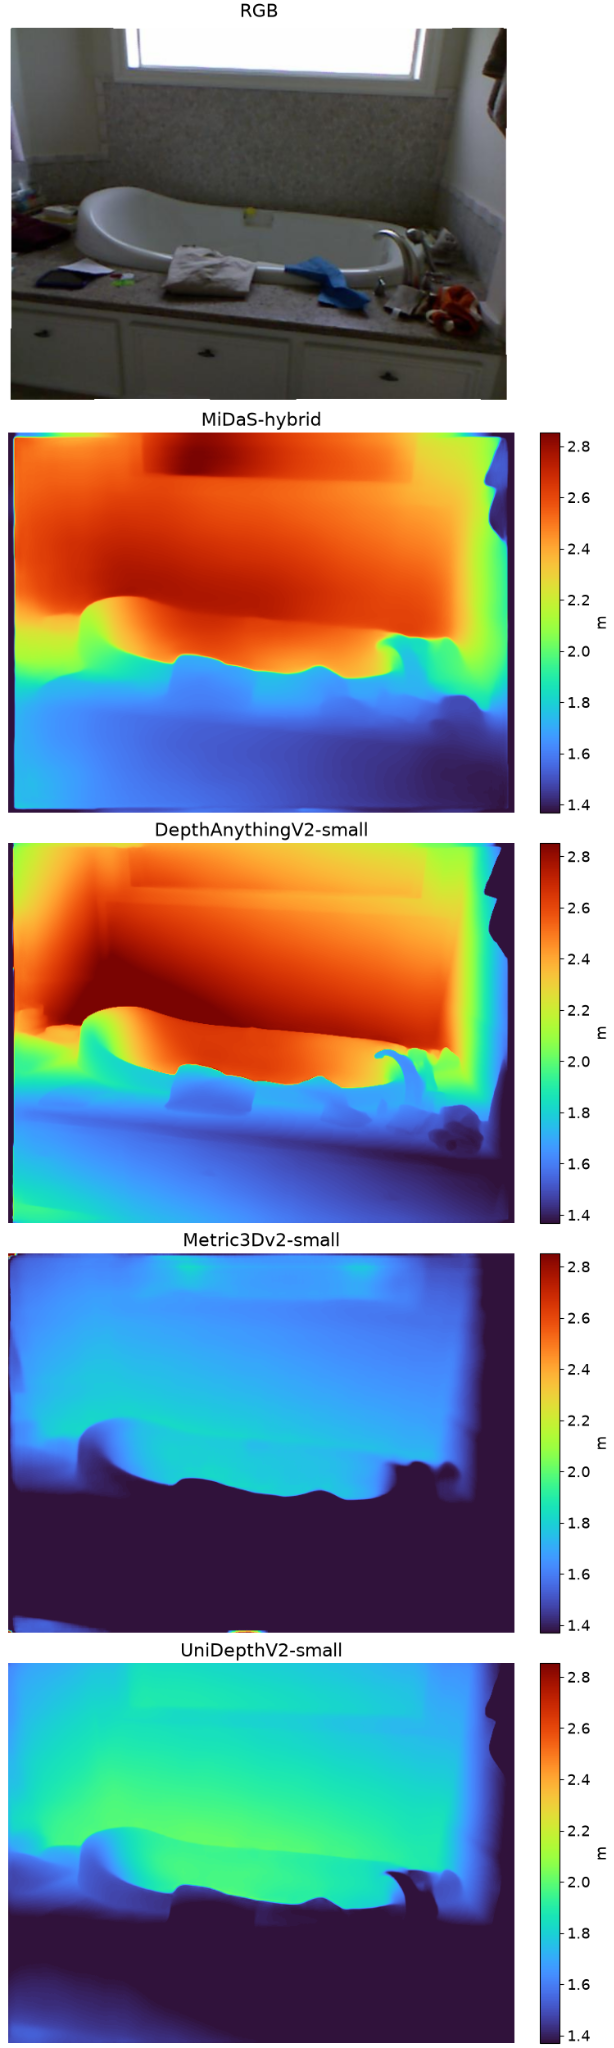
\includegraphics[width=0.75\columnwidth]{fig2.png}
  \caption{Исходное изображение из набора данных и карты глубины для него, предсказанные моделями MiDaS DPT-Hybrid и Depth Anything V2 Small (после согласования масштаба и сдвига), Metric3D v2 ViT-Small и UniDepth V2 Small (без согласования)}
  \label{fig:maps}
\end{figure}

\newpage
\section*{Заключение}

В результате исследования были сравнены четыре современные архитектуры моделей машинного зрения, предсказывающих глубину сцены по монокулярному изображению, оценена их попиксельная ошибка и способность корректно распознавать плоские участки. Основываясь на полученных измерениях, UniDepth V2 является наиболее подходящей для прикладных задач, сочетая в себе скорость обработки кадров и высокую точность предсказаний и не занимая при этом существенно больший объём ОЗУ.

\begin{thebibliography}{9}

\bibitem{pub1} R. Ranftl, K. Lasinger, D. Hafner, K. Schindler and V. Koltun, ``Towards Robust Monocular Depth Estimation: Mixing Datasets for Zero-Shot Cross-Dataset Transfer,'' \textit{IEEE Transactions on Pattern Analysis and Machine Intelligence}, vol. 44, no. 3, pp. 1623--1637, 2022, doi: 10.1109/TPAMI.2020.3019967.

\bibitem{pub2} L. Yang, B. Kang, Z. Huang, Z. Zhao, X. Xu, J. Feng and H. Zhao, ``Depth Anything V2,'' \textit{Advances in Neural Information Processing Systems (NeurIPS)}, 2024. arXiv:2406.09414. Available at: \url{https://arxiv.org/abs/2406.09414} (Accessed: 09.09.2026).

\bibitem{pub3} M. Hu, W. Yin, C. Zhang, Z. Cai, X. Long, H. Chen, K. Wang, G. Yu, C. Shen and S. Shen, ``Metric3D v2: A Versatile Monocular Geometric Foundation Model for Zero-Shot Metric Depth and Surface Normal Estimation,'' \textit{IEEE Transactions on Pattern Analysis and Machine Intelligence}, 2024, doi: 10.1109/TPAMI.2024.3444912. arXiv:2404.15506.

\bibitem{pub4} L. Piccinelli, Y.-H. Yang, C. Sakaridis, M. Segu, S. Li, L. Van Gool and F. Yu, ``UniDepth: Universal Monocular Metric Depth Estimation,'' \textit{Proceedings of the IEEE/CVF Conference on Computer Vision and Pattern Recognition (CVPR)}, 2024, pp. 10106--10116. arXiv:2403.18913.

\bibitem{pub5} N. Silberman, D. Hoiem, P. Kohli and R. Fergus, ``Indoor Segmentation and Support Inference from RGBD Images,'' \textit{European Conference on Computer Vision (ECCV)}, 2012, pp. 746--760.

\bibitem{pub6} М. С. Гришечкин, М. Л. Сульповар, К. А. Проскуряков, «Построение карты пространства по данным стереокамеры в задаче движения мобильного робота»: Сборник статей научно-технического семинара студентов кафедры «Инженерной кибернетики», Москва, 26 июня 2026 года. --- Москва: Национальный исследовательский технологический университет «МИСИС», 2026. --- С. 22--27.

\bibitem{pub7} R. N. Sadekov and D. B. Pazychev, ``Development of a navigation system for UAV based on computer vision,'' \textit{IOP Conf. Ser.: Mater. Sci. Eng.}, vol. 1029, no. 1, p. 012040, 2021, doi: 10.1088/1757-899X/1029/1/012040.

\bibitem{pub8} А. А. Журавлева, А. Э. Цыканов, «Построение интерактивных 3D-туров помещений на основе 3D Gaussian Splatting по изображениям с RGB-камеры»: Сборник статей научно-технического семинара студентов кафедры «Инженерной кибернетики», Москва, 26 июня 2026 года. --- Москва: Национальный исследовательский технологический университет «МИСИС», 2026. --- С. 42--50.

\newpage
\bibitem{pub9} Improving the Accuracy of Supporting Mobile Objects with the Use of the Algorithm of Complex Processing of Signals with a Monocular Camera and LiDAR / R. R. Bikmaev, M. D. Zolotov, A. N. Popov, R. N. Sadekov // 26th Saint Petersburg International Conference on Integrated Navigation Systems, ICINS 2019 -- Proceedings: 26, Saint Petersburg, 27--29 мая 2019 года. -- Saint Petersburg, 2019. -- P. 8769360. -- DOI 10.23919/ICINS.2019.8769360. -- EDN VLZBSK

\end{thebibliography}

\end{document}
